% !TeX spellcheck = de_DE
\documentclass[12pt]{article}
\usepackage[utf8]{inputenc}
\usepackage{geometry}
\usepackage{svg}
\usepackage{float}
\usepackage{caption}
\usepackage{amsmath,amsthm,amsfonts,amssymb,amscd}
\usepackage{fancyhdr}
\usepackage{titlesec}
\usepackage{hyperref}
\usepackage{listings}
\usepackage{booktabs}
\usepackage[skip=3pt]{parskip}
\usepackage[ngerman]{babel}
\pagestyle{empty}
\titleformat*{\section}{\large\bfseries}
\titleformat*{\subsection}{\bfseries}

%
\geometry{
	a4paper,
	total={170mm,240mm},
	left=20mm,
	top=30mm,
}

\date{}
%Bitte ausfüllen
\newcommand\course{Heterogenious Computing}
\newcommand\hwnumber{\large Abschlussprojekt}
\newcommand\Name{Fabian Sponholz}
\newcommand\Neptun{1561546}

%Matheinheiten
\newcommand\m{\:\textrm{m}}
\newcommand\M{\:\Big[\textrm{m}\Big]}
\newcommand\mm{\:\textrm{mm}}
\newcommand\MM{\:\Big[\textrm{mm}\Big]}
\newcommand\un{\underline}
\newcommand\s{\:\textrm{s}}
\newcommand\bS{\:\Big[\textrm{S}\Big]}
\newcommand\ms{\:\frac{\textrm{m}}{\textrm{s}}}
\newcommand\MS{\:\Big[\frac{\textrm{m}}{\textrm{s}}\Big]}
\newcommand\mss{\:\frac{\textrm{m}}{\textrm{s}^2}}
\newcommand\MSS{\:\Big[\frac{\textrm{m}}{\textrm{s}^2}\Big]}

%Trennlinie
\newcommand\separator{\rule{\linewidth}{0.5pt}}

%Bitte nicht einstellen
\renewcommand{\figurename}{Abbildung}
\renewcommand{\tablename}{Tabelle}
\pagestyle{fancyplain}
\headheight 35pt
\lhead{\Name\\\Neptun}
\chead{\textbf{ \hwnumber}}
\rhead{\course \\ \today}
\lfoot{}
\cfoot{}
\rfoot{\small\thepage}
\headsep 1.5em

\begin{document}
	\section*{Einleitung}
	In der Vorlesung \emph{Heterogenious Computing} haben wir uns auch mit dem Programmieren von Grafikkarten befasst und dort verschiedene Schnittstellen kennengelernt, die es ermöglichen, Code direkt auf solcher Hardware auszuführen.
	Insbesondere gut parallelisierbare Aufgaben lassen sich so erheblich beschleunigen im Vergleich zur Ausführung auf einer CPU.
	Zunächst wäre da einmal \emph{OpenCL} zu nennen, welches eine offene Schnittstelle für verschiedenste Geräte wie FPGAs, CPUs und GPUs darstellt.
	Zusätzlich gibt es bei GPUs noch herstellereigene Schnittstellen wie z.B. \emph{Nvidia CUDA} oder \emph{Intel oneAPI}, die grundsätzlich ähnliche Funktionalitäten bieten.
	
	Für mein Abschlussprojekt stelle ich mir die Frage, ob die Verwendung von herstellerspezifischen APIs im Vergleich zu OpenCL einen signifikanten Performance-Vorteil bringt.
	Dazu möchte ich je einen rechenintensiven Algorithmus zur Messung der Rechenleistung und einen speicherintensiven Algorithmus zur Messung der Speicherbandbreite implementieren.
	Diese Algorithmen werde ich für verschiedene Schnittstellen anpassen und so die Performance (Laufzeit) vergleichen.
	
	\subsection*{Gewählte Algorithmen}
	Folgende Algorithmen habe ich für das Experiment ausgewählt:
	
	\begin{itemize}
		\item \textbf{Matrix-Multiplikation} ist eine einfache aber rechenintensive Operation, die sich leicht parallelisieren lässt. Durch die Größe der Matrizen lässt sich außerdem die Arbeitslast gut skalieren.
		\item \textbf{Kopieren von Arrays} ist eine Operation, die wenig Rechenleistung benötigt, aber die Speicherbandbreite stark auslastet. Zudem lässt sich hier die Arbeitslast ebenfalls gut durch die Größe des Arrays skalieren.
	\end{itemize}
	
	\section*{Implementierungsdetails}
	\subsection*{Generelles}
	Die oben genannten APIs verwenden sogenannte Command-Queues, um unter anderem Kopier-Operationen asynchron zu verarbeiten.
	Da ich nur die Laufzeit des tatsächlichen Kernel-Pro-gramms messen möchte und die Zeit, die das Kopieren vom/zum Host ausgespart werden soll, ist es wichtig sicherzustellen, dass diese Operationen vor Beginn der Zeitmessung abgeschlossen sind.
	Glücklicherweise gibt es dafür passende Funktionen, wie z.B. \texttt{queue.flush()} bei OpenCL oder eine synchrone Kopier-Methode \texttt{Driver.memcpy\_htod} bei CUDA.
	Auch die eigentliche Ausführung der Kernels findet normalerweise asynchron statt, hier kann bei OpenCL zur Synchronisierung eine \texttt{wait()}-Methode aufgerufen werden, bei CUDA kann der selbe Effekt durch einen Aufruf von \texttt{Context.synchronize()} erzielt werden.
	
	\subsection*{Matrix-Multiplikation}
	Hier werden als Eingabe zwei zufällig generierte 10000x10000-Matrizen verwendet, die dann naiv multipliziert werden. Hier berechnet jede Arbeitseinheit auf der GPU ein Feld der resultierenden Matrix.
	Da hier das Kopieren der Daten nur einen winzigen Bruchteil der Laufzeit ausmacht, wird das Ergebnis zurückgeschrieben und teilweise ausgegeben.
	Die Laufzeitmessung beschränkt sich allerdings trotzdem nur auf die eigentliche Berechnung.
	
	Das Programm wird 100 mal iteriert, wobei hier jedes mal die selben Operanden verwendet werden: Zu Beginn werden die Eingabematrizen erstellt und auf die GPU kopiert, dann wird die Berechnung 100 mal wiederholt.
	
	\subsection*{Copy-Kernel}
	Als Eingabe wird hier ein Array von 32-Bit Floats verwendet, wobei jede Arbeitseinheit je eine der Zahlen in ein gleich großes Ausgabearray kopiert.
	Die Größe des Arrays wird an den verfügbaren GPU-Speicher angepasst, um diesen optimal auszunutzen.
	Hier ist es besonders wichtig, die Kopiervorgänge zur GPU nicht in die Zeitmessung mit aufzunehmen, da diese deutlich länger dauern als die Kernelausführung.
	
	\section*{Testsysteme}
	Hier kurz die technischen Daten der Grafikkarten, die ich in meinem Test verwendet habe:
	
	\subsection*{Testsystem 1: NVIDIA}
	\begin{tabular}{@{}ll@{}}
		\toprule
		\textbf{Eigenschaft}             & \textbf{Wert}                      \\ \midrule
		\textbf{Bezeichnung}			& NVidia GeForce RTX 2060			\\
		\textbf{GPU-Kerne (CUDA Cores)} & 1920                               \\
		\textbf{Basistakt}              & 1365 MHz                           \\
		\textbf{Boost-Takt}             & 1680 MHz                           \\
		\textbf{Speichergröße}          & 6 GB GDDR6                         \\
		\textbf{Speicherinterface}      & 192 Bit                            \\
		\textbf{Speicherbandbreite}     & 336 GB/s                           \\
		\textbf{Speichertakt}           & 1750 MHz (14 Gbps effektiv)        \\
		\bottomrule
	\end{tabular}
	
	\subsection*{Testsystem 2: Intel}
	\begin{tabular}{@{}ll@{}}
		\toprule
		\textbf{Eigenschaft}             & \textbf{Wert}                         \\ \midrule
		\textbf{Bezeichnung}		     & Intel Arc A770 (Limited Edition)		\\
		\textbf{GPU-Kerne (Shader)}      & 4096                                   \\
		\textbf{Basistakt}               & 2100 MHz                              \\
		\textbf{Boost-Takt}              & 2400 MHz                       		\\
		\textbf{Speichergröße}           & 16 GB GDDR6                           \\
		\textbf{Speicherinterface}       & 256 Bit                               \\
		\textbf{Speicherbandbreite}      & 560 GB/s                              \\
		\textbf{Speichertakt}            & 2000 MHz (16 Gbps effektiv)            \\
		\bottomrule
	\end{tabular}
	
	\section*{Auswertung Testsystem 1}
	Für die Zeitmessung habe ich die Python-Funktion \texttt{time.perf\_counter\_ns()} verwendet, um eine Zeitmessung in Nanosekunden vorzunehmen.
	Die erhaltenen Werte habe ich dann in eine Liste geschrieben, die ich dann in R weiter auswerten konnte.
	Im Folgenden lege ich die Ergebnisse der Zeitmessungen für den Vergleich zwischen OpenCL und CUDA auf Testsystem 1 dar.
	
	\subsection*{Ergebnisse: Matrix-Multiplikation}
	\subsubsection*{OpenCL}
	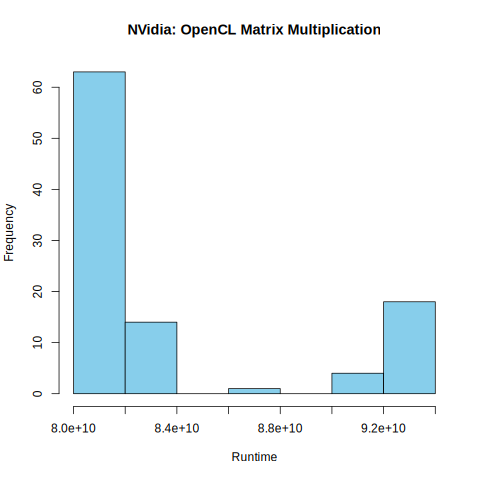
\includegraphics[width=0.5\textwidth]{../statistics/nvidia/opencl/histogram_matmul.png}
	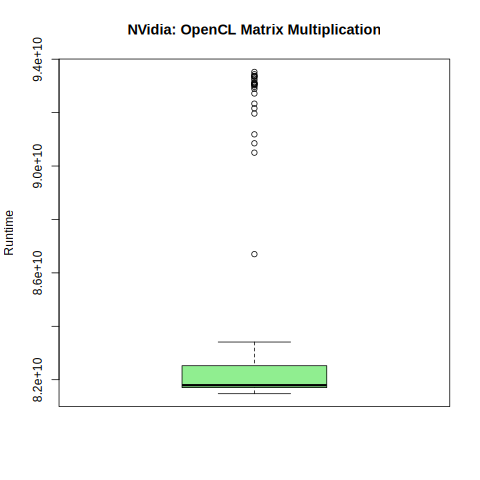
\includegraphics[width=0.5\textwidth]{../statistics/nvidia/opencl/boxplot_matmul.png}
	\\
	\begin{center}
		\begin{tabular}{|l|l|}
		\toprule
		\textbf{Mittlere Laufzeit} 		& $84.27s$ \\
		\textbf{1. Quartil}				& $81.70s$ \\
		\textbf{Median}					& $81.79s$  \\
		\textbf{3. Quartil}				& $82.49s$  \\
		\bottomrule
		\end{tabular}
	\end{center}
	
	\subsubsection*{CUDA}
	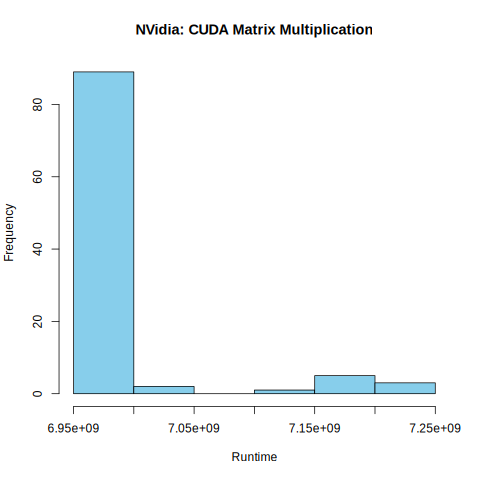
\includegraphics[width=0.5\textwidth]{../statistics/nvidia/cuda/histogram_matmul.png}
	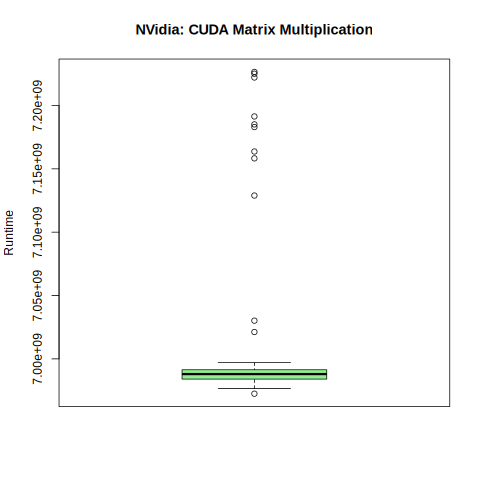
\includegraphics[width=0.5\textwidth]{../statistics/nvidia/cuda/boxplot_matmul.png}
	\\
	\begin{center}
		\begin{tabular}{|l|l|}
			\toprule
			\textbf{Mittlere Laufzeit} 		& $7.00s$ \\
			\textbf{1. Quartil}				& $6.98s$ \\
			\textbf{Median}					& $6.99s$  \\
			\textbf{3. Quartil}				& $6.99s$  \\
			\bottomrule
		\end{tabular}
	\end{center}
	\medskip
	
	Dieses Ergebnis hat mich wirklich erstaunt. 
	Die Laufzeit mit CUDA ist hier, obwohl der Algorithmus der selbe ist und sich die Kernel-Codes entsprechend sehr ähnlich sehen, um eine Zehnerpotenz schneller als mit OpenCL!
	Außerdem sieht man, dass die Laufzeiten von Durchlauf zu Durchlauf recht ähnlich sind und es nur wenige Ausreißer nach oben gibt.
	
	Ich habe auch die Leistungsdaten der Grafikkarte während der Tests beobachtet, wobei ich auch gesehen habe, dass die Leistungsaufnahme während dem Durchlauf der CUDA-Implementierung etwa 20\% höher war als bei der OpenCL-Variante.
	
	

	\subsection*{Ergebnisse: Copy Kernel}
	\subsubsection*{OpenCL}
	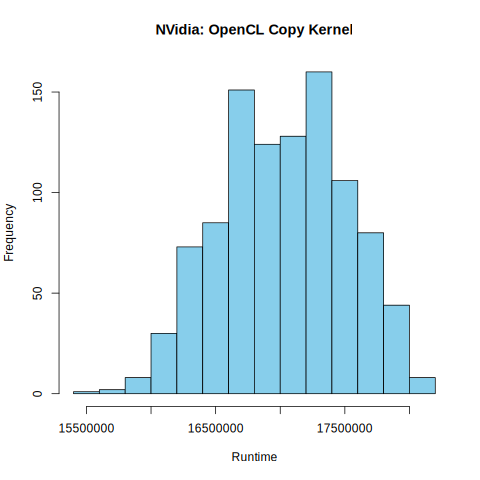
\includegraphics[width=0.5\textwidth]{../statistics/nvidia/opencl/histogram_copy.png}
	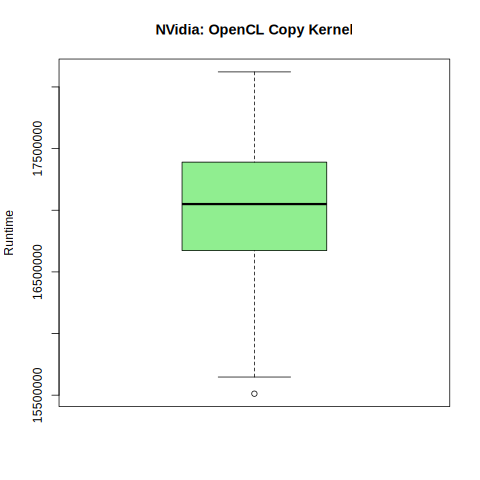
\includegraphics[width=0.5\textwidth]{../statistics/nvidia/opencl/boxplot_copy.png}
	\\
	\begin{center}
		\begin{tabular}{|l|l|}
			\toprule
			\textbf{Mittlere Laufzeit} 		& $17.02ms$ \\
			\textbf{1. Quartil}				& $16.67ms$ \\
			\textbf{Median}					& $17.02ms$  \\
			\textbf{3. Quartil}				& $17.39ms$  \\
			\bottomrule
		\end{tabular}
	\end{center}
	
	\subsubsection*{CUDA}
	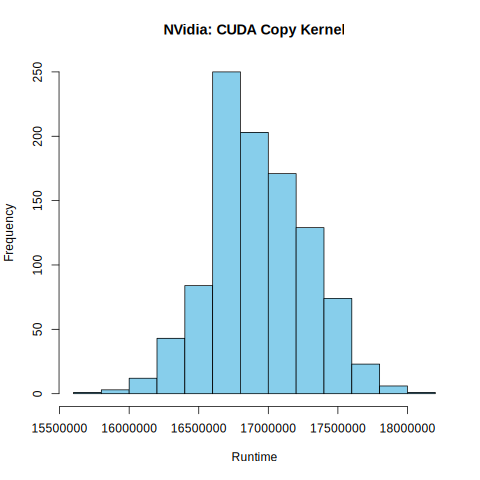
\includegraphics[width=0.5\textwidth]{../statistics/nvidia/cuda/histogram_copy.png}
	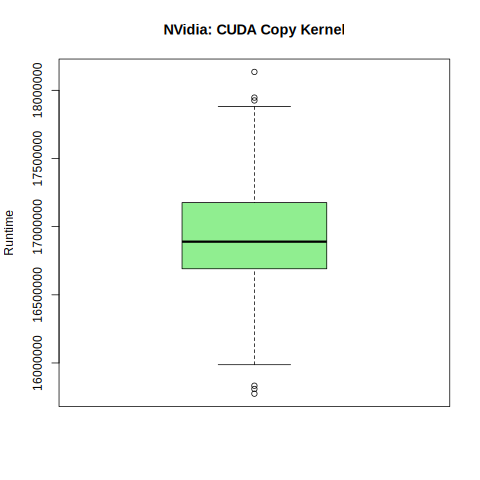
\includegraphics[width=0.5\textwidth]{../statistics/nvidia/cuda/boxplot_copy.png}
	\\
	\begin{center}
		\begin{tabular}{|l|l|}
			\toprule
			\textbf{Mittlere Laufzeit} 		& $16.93ms$ \\
			\textbf{1. Quartil}				& $16.69ms$ \\
			\textbf{Median}					& $16.89ms$  \\
			\textbf{3. Quartil}				& $17.18ms$  \\
			\bottomrule
		\end{tabular}
	\end{center}
	\medskip
	Auch hier zeigt sich eine sehr kleine Abweichung zugunsten von CUDA, jedoch ist diese so gering, dass ich sie für irrelevant halte.
	Außerdem wird hier im Histogramm annähernd eine Normalverteilung ersichtlich, während diese im ersten Versuch aufgrund der starken Ausreißer nicht erkennbar ist.
	
	\section*{Auswertung Testsystem 2}
	Für die OpenCL-Tests habe ich hier den selben Python-Code verwendet wie bereits bei Testsystem 1, um auch einen Vergleich zwischen den beiden Systemen zu ermöglichen.
	Auch die Dimensionen der Eingabedaten habe ich gleich gelassen.
	
	Leider habe ich es nicht geschafft, die Python-Schnittstelle von oneAPI zum Laufen zu bringen, daher habe ich für die oneAPI-Tests stattdessen äquivalente Programme in C++ erstellt.
	Da der eigentliche Code sowieso nicht in Python ausgeführt wird, sollte der Einfluss auf die Ergebnisse nicht relevant sein.
	Für die Laufzeitmessung habe ich das eingebaute Profiling-Tool von oneAPI verwendet, da dies hier die beste Möglichkeit ist, die reine Kernel-Laufzeit zu messen.
	
	\subsection*{Ergebnisse: Matrix-Multiplikation}
	\subsubsection*{OpenCL}
	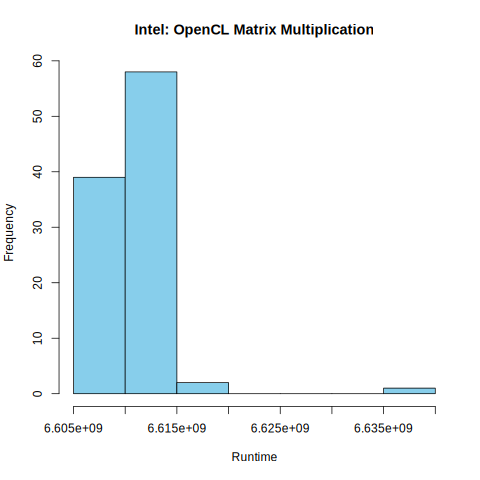
\includegraphics[width=0.5\textwidth]{../statistics/intel/opencl/histogram_matmul.png}
	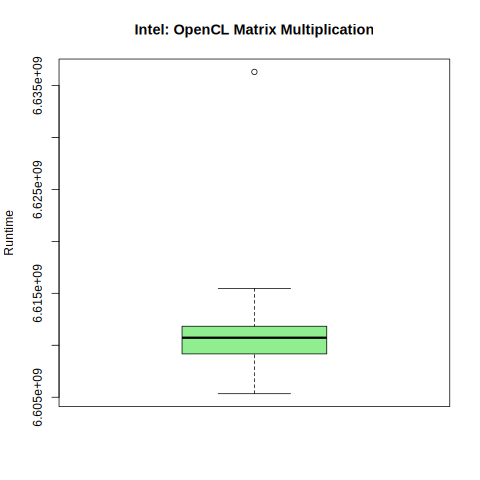
\includegraphics[width=0.5\textwidth]{../statistics/intel/opencl/boxplot_matmul.png}
	\\
	\begin{center}
		\begin{tabular}{|l|l|}
			\toprule
			\textbf{Mittlere Laufzeit} 		& $6.61s$ \\
			\textbf{1. Quartil}				& $6.61s$ \\
			\textbf{Median}					& $6.61s$  \\
			\textbf{3. Quartil}				& $6.61s$  \\
			\bottomrule
		\end{tabular}
	\end{center}
	
	\subsubsection*{oneAPI}
	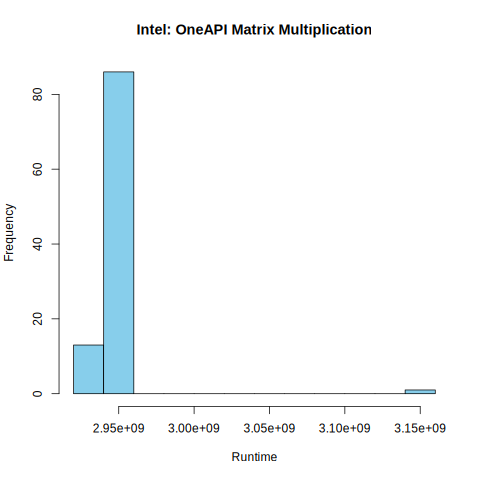
\includegraphics[width=0.5\textwidth]{../statistics/intel/oneapi/histogram_matmul.png}
	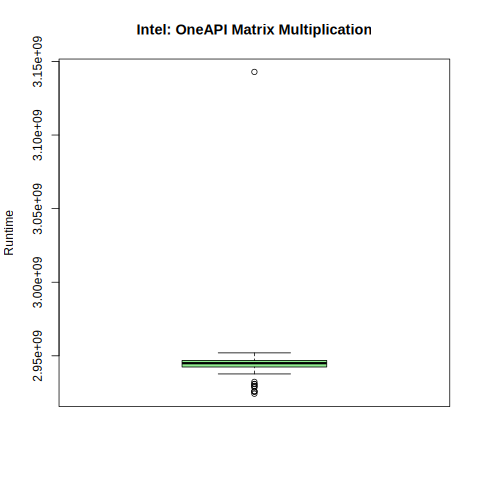
\includegraphics[width=0.5\textwidth]{../statistics/intel/oneapi/boxplot_matmul.png}
	\\
	\begin{center}
		\begin{tabular}{|l|l|}
			\toprule
			\textbf{Mittlere Laufzeit} 		& $2.95s$ \\
			\textbf{1. Quartil}				& $2.94s$ \\
			\textbf{Median}					& $2.95s$  \\
			\textbf{3. Quartil}				& $2.95s$  \\
			\bottomrule
		\end{tabular}
	\end{center}
	\medskip
	
	Ebenso wie bei Testsystem 1 zeigt sich hier ein signifikanter Performance-Unterschied zwischen OpenCL und der herstellereigenen Schnittstelle.
	Zwar ist der Speedup hier mit \glqq nur\grqq{} etwa zwei deutlich geringer als beim Testsystem 1, jedoch ist das immer noch ein erheblich besseres Ergebnis.
	Welchen Einfluss die Verwendung von Intels Profiling-Tool anstelle einer Host-Basierten Zeitmessung hat, lässt sich so erstmal nicht herausfinden; Der Unterschied sollte allerdings so gering sein, dass er das Ergebnis in seiner Aussagekraft nicht weiter verändern würde.
	
	Interessant ist auch, dass Ausreißer viel seltener sind und außerdem in erster Linie ein einziger Ausreißer zu Beginn des Testlaufs heraussticht.
	Dies deutet auf eine gewisse Initialisierungsphase hin, die die Intel-Grafikkarte sowohl bei Verwendung von OpenCL als auch bei oneAPI durchzuführen scheint.
	Grundsätzlich sind die einzelnen Datenpunkte aber viel weniger gestreut als bei Testsystem 1.
	
	Zuletzt fällt noch auf, dass die Performance von Testsystem 1 mit CUDA und Testsystem 2 mit OpenCL bei der Matrix-Multiplikation fast auf Augenhöhe ist.
	Da die Grafikkarte von Testsystem 2 in der Theorie bedeutend stärker ist als die von Testsystem 1, ist das höchst interessant und unterstreicht die höhere Effizienz von CUDA im Vergleich zu OpenCL.

	\subsection*{Ergebnisse: Copy Kernel}	
	\subsubsection*{OpenCL}
	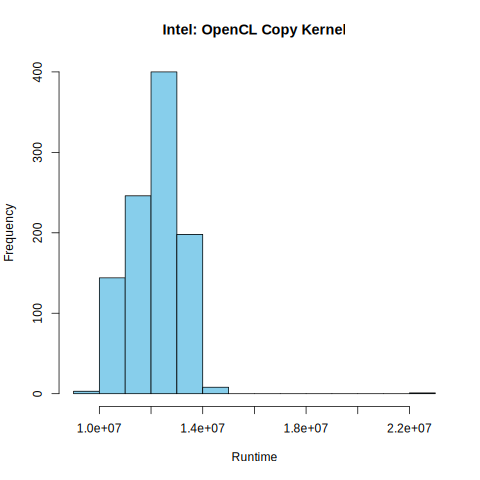
\includegraphics[width=0.5\textwidth]{../statistics/intel/opencl/histogram_copy.png}
	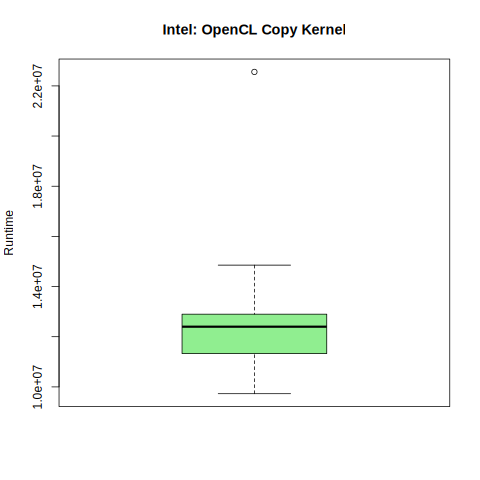
\includegraphics[width=0.5\textwidth]{../statistics/intel/opencl/boxplot_copy.png}
	\\
	\begin{center}
		\begin{tabular}{|l|l|}
			\toprule
			\textbf{Mittlere Laufzeit} 		& $12.20ms$ \\
			\textbf{1. Quartil}				& $11.33ms$ \\
			\textbf{Median}					& $12.40ms$  \\
			\textbf{3. Quartil}				& $12.90ms$  \\
			\bottomrule
		\end{tabular}
	\end{center}
	
	\subsubsection*{oneAPI}
	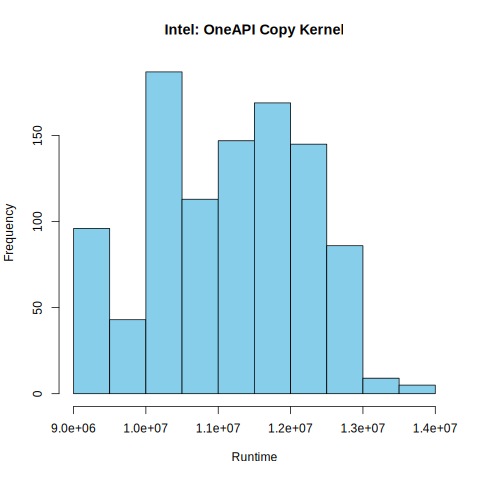
\includegraphics[width=0.5\textwidth]{../statistics/intel/oneapi/histogram_copy.png}
	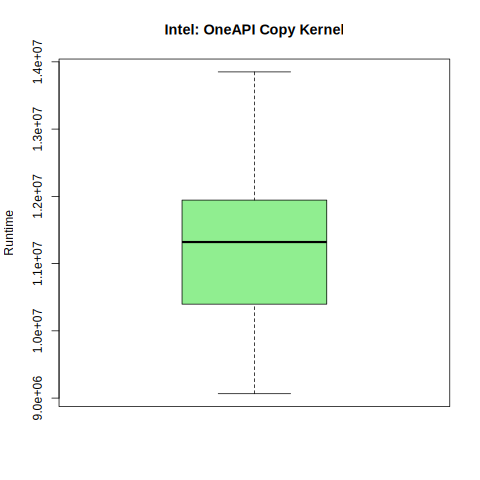
\includegraphics[width=0.5\textwidth]{../statistics/intel/oneapi/boxplot_copy.png}
	\\
	\begin{center}
		\begin{tabular}{|l|l|}
			\toprule
			\textbf{Mittlere Laufzeit} 		& $11.15ms$ \\
			\textbf{1. Quartil}				& $10.40ms$ \\
			\textbf{Median}					& $11.32ms$  \\
			\textbf{3. Quartil}				& $11.94ms$  \\
			\bottomrule
		\end{tabular}
	\end{center}
	\medskip
	
	Auch hier wiederholt sich das Bild aus dem Ergebnis von Testsystem 1.
	Die Verwendung von oneAPI bringt hier einen Speedup von etwa 10\% und ist daher etwas größer als bei Testsystem 1.
	Trotzdem ist der Effekt hier lange nicht so groß, wie bei der Matrix-Multiplikation.
	
	\section*{Zusammenfassung}
	Zusammenfassend lässt sich sagen, dass die Verwendung von herstellerspezifischen APIs im Vergleich zu OpenCL insbesondere bei Compute-Lastigen Aufgaben \textbf{einen erheblichen Speedup} bringen kann.
	Möglicherweise ist es durch Optimierungen am OpenCL-Code hinsichtlich der verwendeten Speicherbereiche möglich, das Ergebnis zu Gunsten von OpenCL zu verbessern, jedoch zeigt dieses Experiment, dass bei naiver Implementierung von Compute-Lastigen Algorithmen die Hersteller-APIs nicht durch OpenCL geschlagen werden können.
	
	Auch bei Anwendungen, die in erster Linie die Speicherbandbreite der Grafikkarte auslasten, bringen die herstellerspezifischen APIs mitunter einen Vorteil; dieser scheint jedoch nicht so ausgeprägt zu sein wie bei Compute-Lastigen Anwendungen.
	Möglicherweise gibt es jedoch noch andere Algorithmen, die die Speicherbandbreite noch besser ausnutzen und so einen noch gravierenderen Unterschied feststellen könnten.
	
\end{document}